\documentclass{beamer}
\usepackage{ctex, hyperref}
\usepackage[T1]{fontenc}

% other packages
\usepackage{latexsym,amsmath,xcolor,multicol,booktabs,calligra}
\usepackage{graphicx,pstricks,listings,stackengine}
\usepackage{textcomp}

\author{谭诗弘，黄育民，曹洪珲}
\title{智能系统设计实践}
\subtitle{六足机器人避障控制 第四次进展汇报}
\institute{武汉大学电子信息学院}
\date{2025年11月3日}
\usepackage{whu}

% defs
\def\cmd#1{\texttt{\color{red}\footnotesize $\backslash$#1}}
\def\env#1{\texttt{\color{blue}\footnotesize #1}}
\definecolor{deepblue}{rgb}{0,0,0.5}
\definecolor{deepred}{rgb}{0.6,0,0}
\definecolor{deepgreen}{rgb}{0,0.5,0}
\definecolor{halfgray}{gray}{0.55}

\lstset{
    basicstyle=\ttfamily\small,
    keywordstyle=\bfseries\color{deepblue},
    emphstyle=\ttfamily\color{deepred},    % Custom highlighting style
    stringstyle=\color{deepgreen},
    numbers=left,
    numberstyle=\small\color{halfgray},
    rulesepcolor=\color{red!20!green!20!blue!20},
    frame=shadowbox,
}


\begin{document}

\kaishu
\begin{frame}
    \titlepage
    \begin{figure}[htpb]
        \begin{center}
            
\includegraphics[width=0.2\linewidth]{pic/whulogo.png}
        \end{center}
    \end{figure}
\end{frame}

% \begin{frame}
%     \tableofcontents[sectionstyle=show,subsectionstyle=show/shaded/hide,subsubsectionstyle=show/shaded/hide]
% \end{frame}

\section{本周进展}

\begin{frame}{本周进展}
    \begin{itemize}
        \item 通过代码实现了机器人跨越低矮障碍物。
    \end{itemize}
\end{frame}

\begin{frame}{策略形成}
    \begin{itemize}
        \item 在驱动库内已经定义好关于平地行走相关的代码，因此能够在需要跨越障碍物时由人控制是否跨越，在跨越障碍物的中途由平地行走的三角步态进行管理，当腿部贴近障碍物时，由人控制舵机进行腿部跨越。
        \item 采用跨越障碍物途中小步幅前进的方式，让机器人能够更好地贴近障碍物，从而更好地进行跨越。
    \end{itemize}
\end{frame}

\begin{frame}{实验结果展示}
    \begin{figure}[htpb]
        \centering
        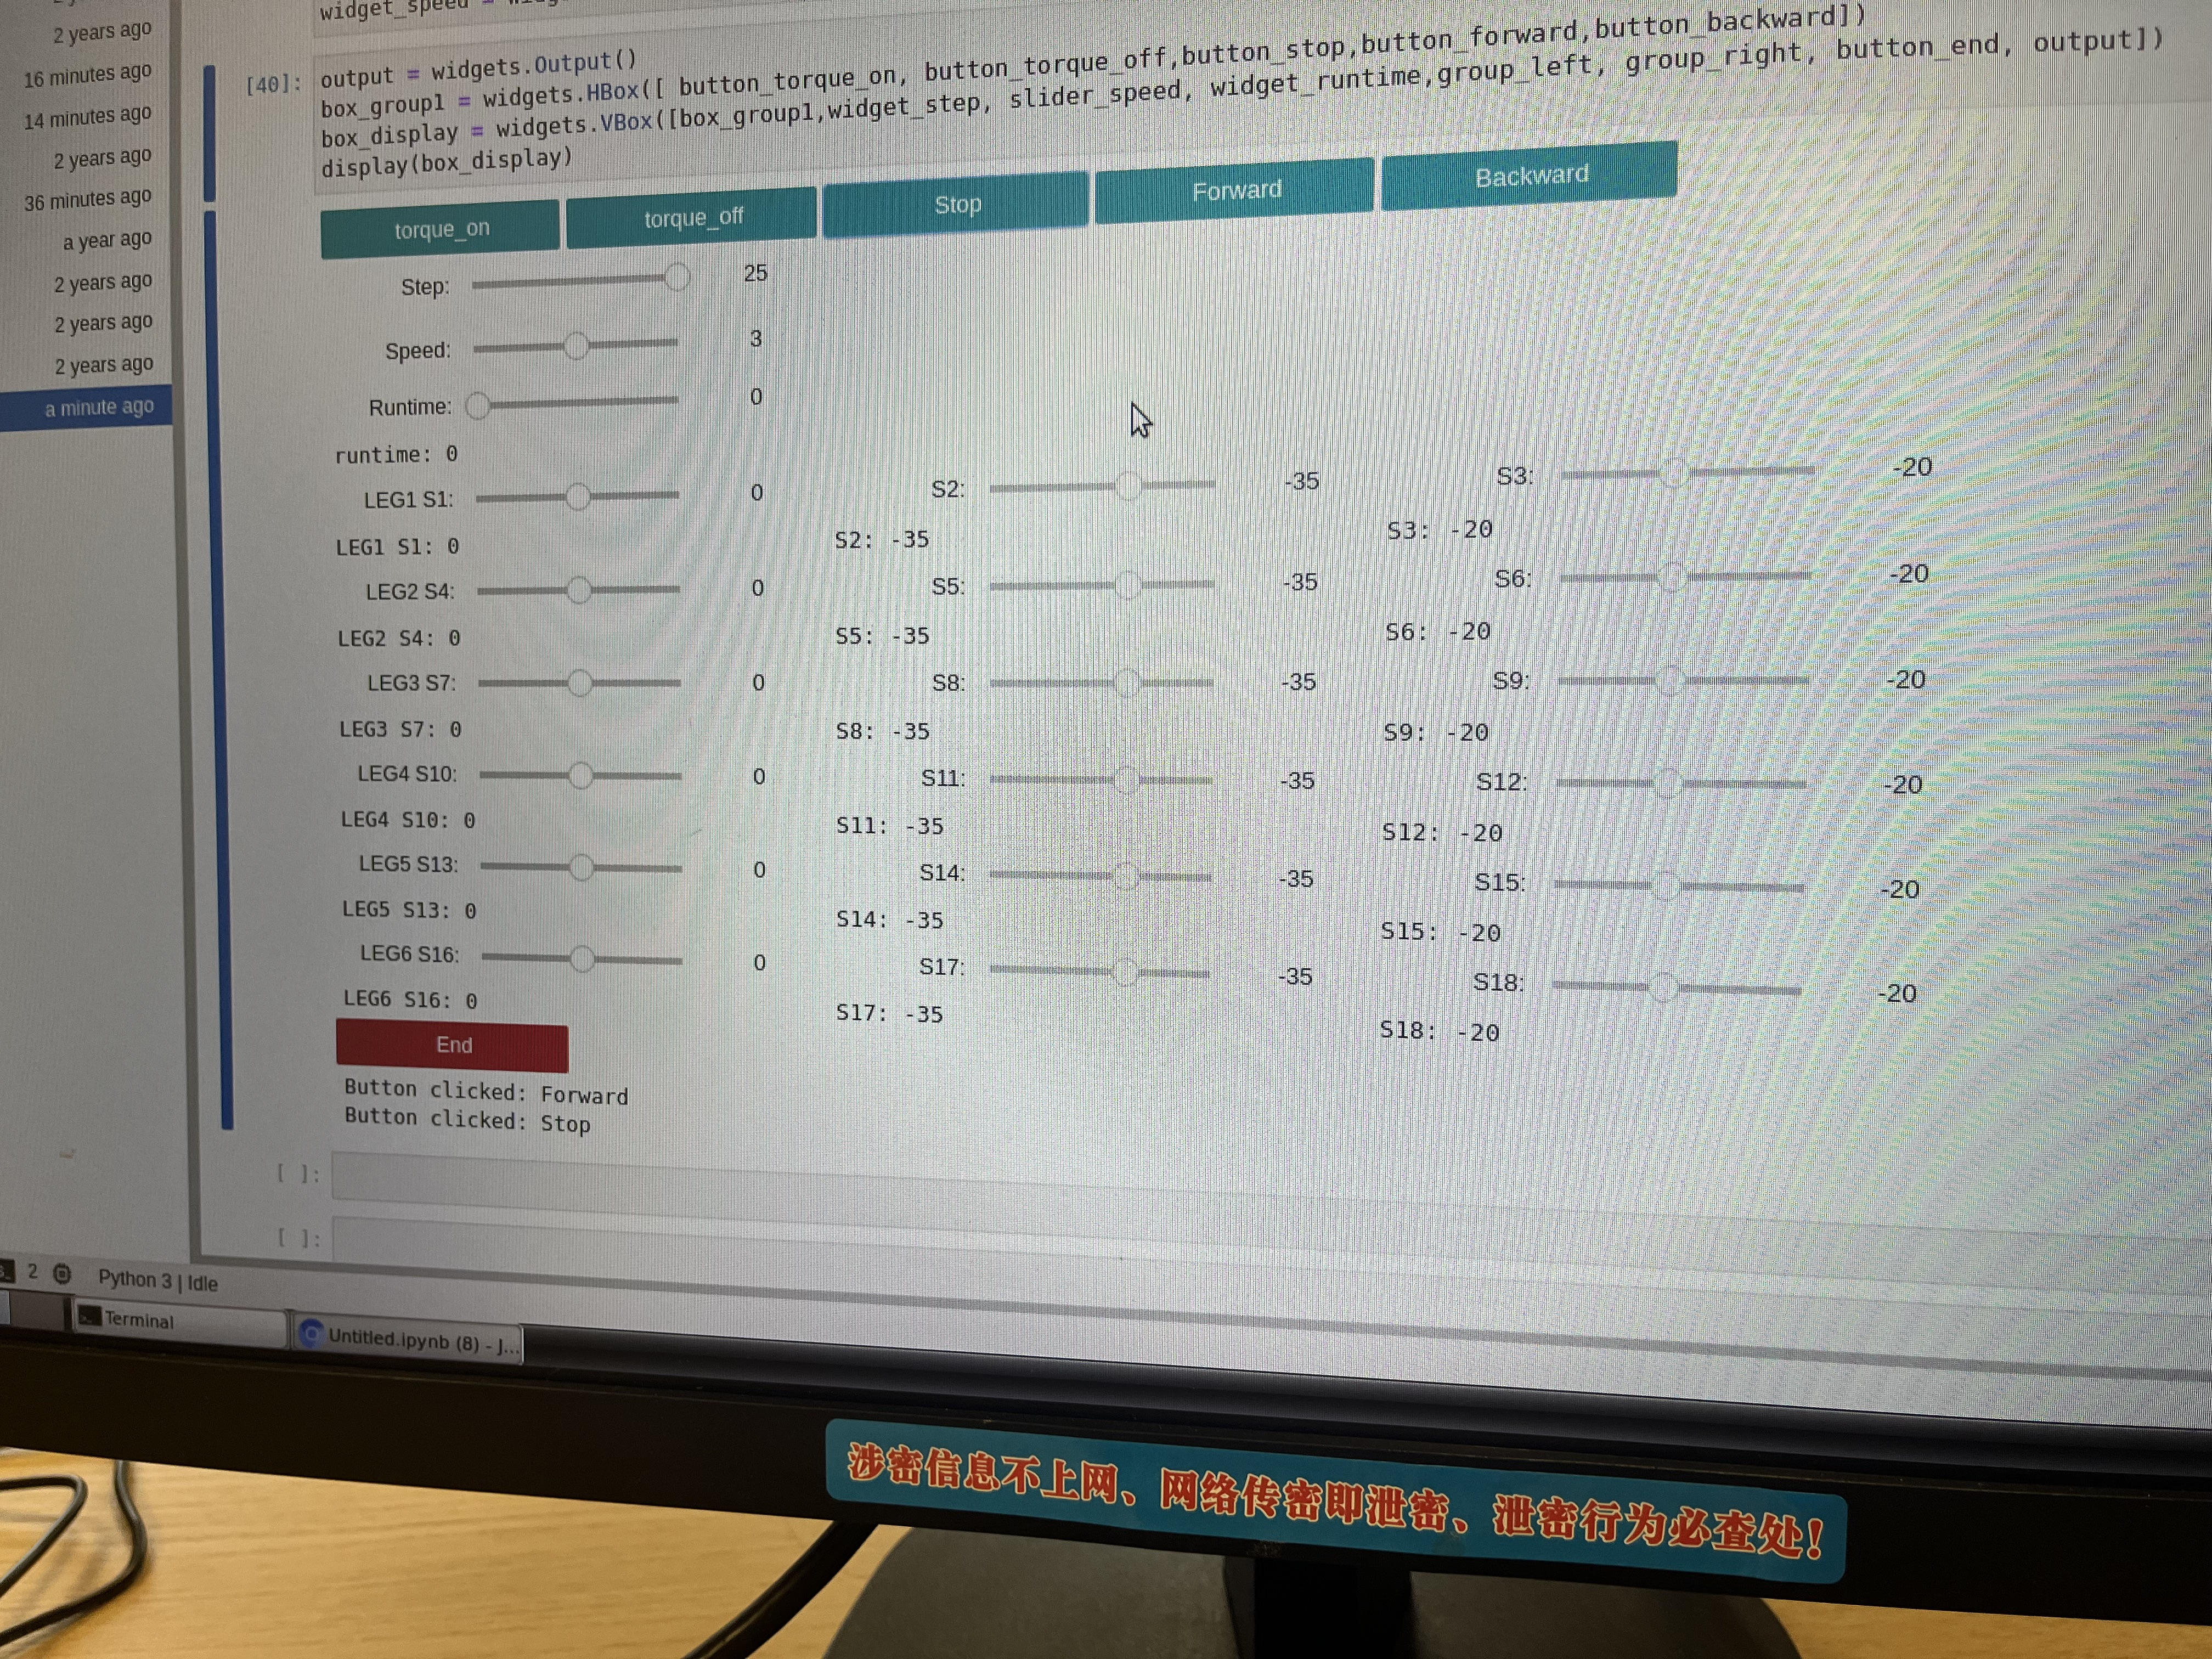
\includegraphics[width=0.8\linewidth]{pic/combi.jpg}
    \end{figure}
\end{frame}

\begin{frame}{实验结果展示}
    \begin{center}
        视频展示
    \end{center}
\end{frame}

\section{后续规划}

\begin{frame}{后续规划}
    \begin{itemize}
        \item 实现人机更友好的障碍物翻越方案。
    \end{itemize}
\end{frame}

\begin{frame}
    \begin{center}
        {\Huge\calligra Thanks!}
    \end{center}
\end{frame}

\end{document}